\chapter{Data, Trigger and Event Selection}

\section{Data}

The search for GMSB described in this thesis uses $1.1 \unit{fb^{-1}}$ of data 
taken from March to June 2011. This corresponds to the data set used for the 
results presented at the International Europhysics Conference in High Energy 
Physics in July 2011. \\

The centre of mass energy of the proton-proton collisions is $7\unit{TeV}$ which
makes the LHC the highest energy particle collider to date. A higher centre of 
mass energy increases the production cross-section of certain processes, for 
example stong production SUSY, and also enables the production of more massive 
particles. It should be noted that the important energy is not the centre of 
mass energy of the proton collision, but that of the parton collision which is 
$\sim 1 \unit{TeV}$ on average. \\

The instantaneous luminosity has increased over the data taking period by 
increasing the intensity of the beams and the number of bunches. Increasing the 
intensity of the beams leads to more interactions per bunch crossing -- an 
effect called pile-up. During the period when this data was taken the luminosity 
was $\sim 10^{33} \unit{cm^{-2}s^{-1}}$. \\

Figure \ref{fig:intlumi} shows the integrated luminosity recorded by CMS over 
time until September 2011. \\

\begin{figure}
\begin{center}
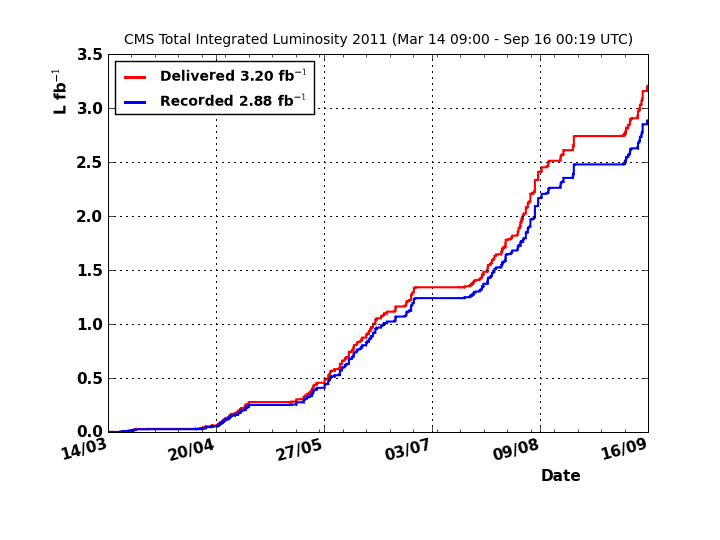
\includegraphics[width=\textwidth]{Integrated_Luminosity.png}
\caption{The integrated luminosity vs time delivered to (red) and recorded by
(blue) CMS during stable beams at $\sqrt{s} = 7 \unit{TeV}$.}
\end{center}
\label{fig:intlumi}
\end{figure}

\section{Monte Carlo Samples}
\label{sec:Monte_Carlo_Samples}

Events of QCD processes, SUSY signal models and Electroweak processes are 
generated using Monte Carlo (MC) techniques followed by detector simulation. The
simulated data gives predictions to be compared with obsevations and used to 
validate analysis methods. The samples are generated using Pythia 6 
\cite{pythia6} and GEANT 4 \cite{geant} is used for the detector simulation. \\

Pile-up is simulated in the MC samples however the MC does not reproduce the 
vertex mutiplicity distribution seen in the data. To correctly simulate pile-up 
the MC is re-weighted to reproduce the number of vertices distribution seen in 
the data. Figure \ref{fig:nVertices} shows the distribution of number of 
vertices in the data and MC. \\

\begin{figure}
\begin{center}
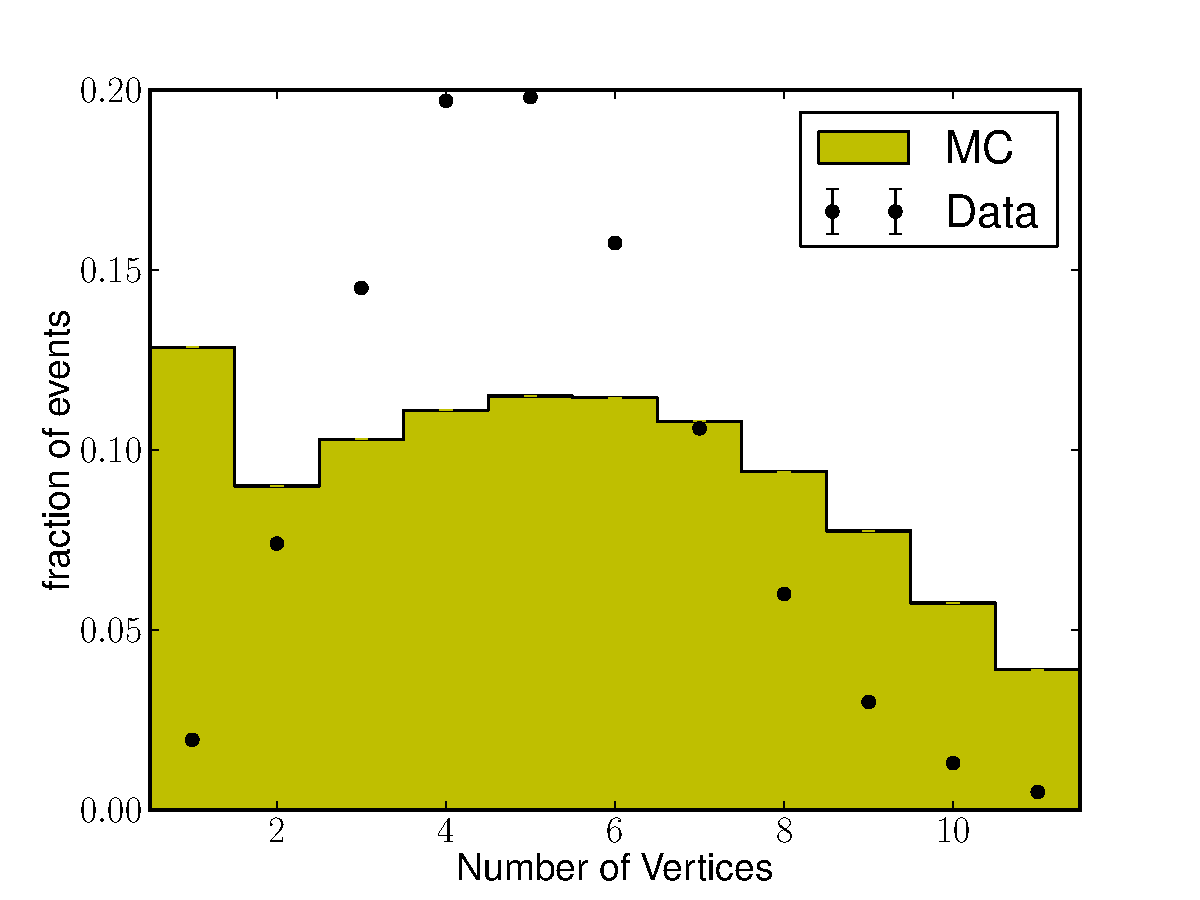
\includegraphics[width=0.8\textwidth]{nVertices.pdf}
\end{center}
%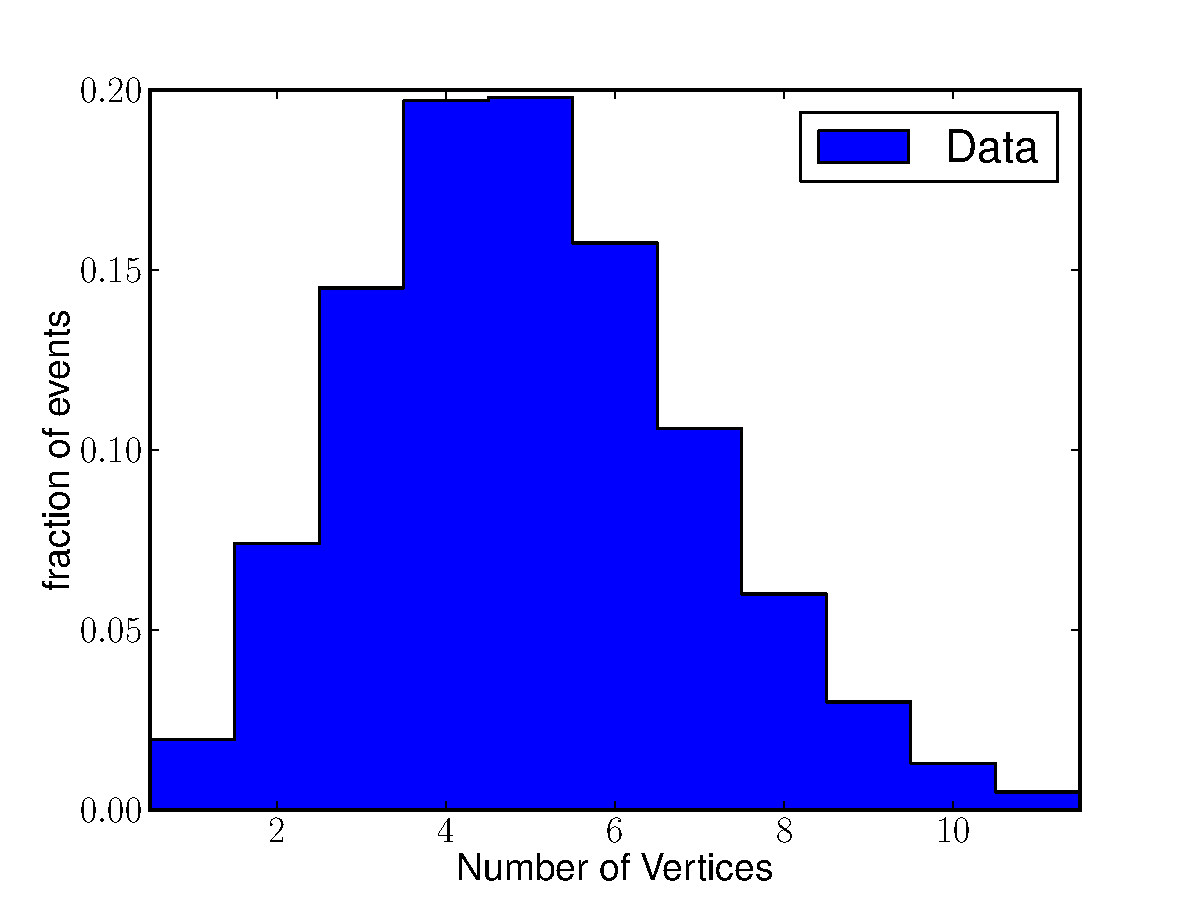
\includegraphics[width=0.5\textwidth]{nVertices_Data.pdf}
%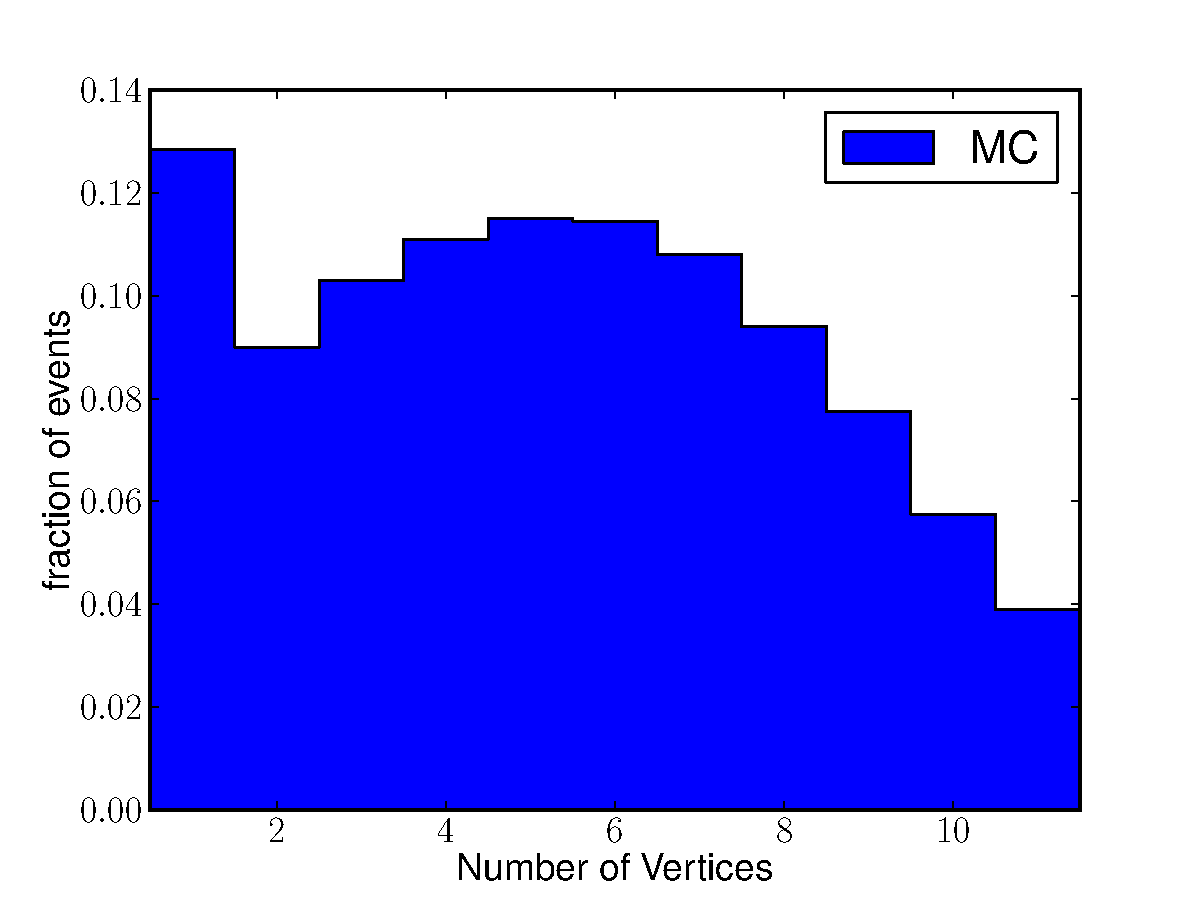
\includegraphics[width=0.5\textwidth]{nVertices_MC.pdf}
%\caption{The distribution of number of vertices in the data (left) and the MC
%(right).}
\caption{The distribution of number of vertices in the data compared to the MC}
\label{fig:nVertices}
\end{figure}

Figure \ref{fig:Data_vs_MC} shows plots of $\HT$ and $\MET$ to show how 
accurately the MC models the data. The prediction is good for $\HT$, but the 
$\MET$ distribution is broader in the data than the MC. This shows that jets 
with $\pT > 40 \unit{GeV}$ are well described by the MC, but lower energy jets 
and unclustered energy are less well modelled. \\

\begin{figure}
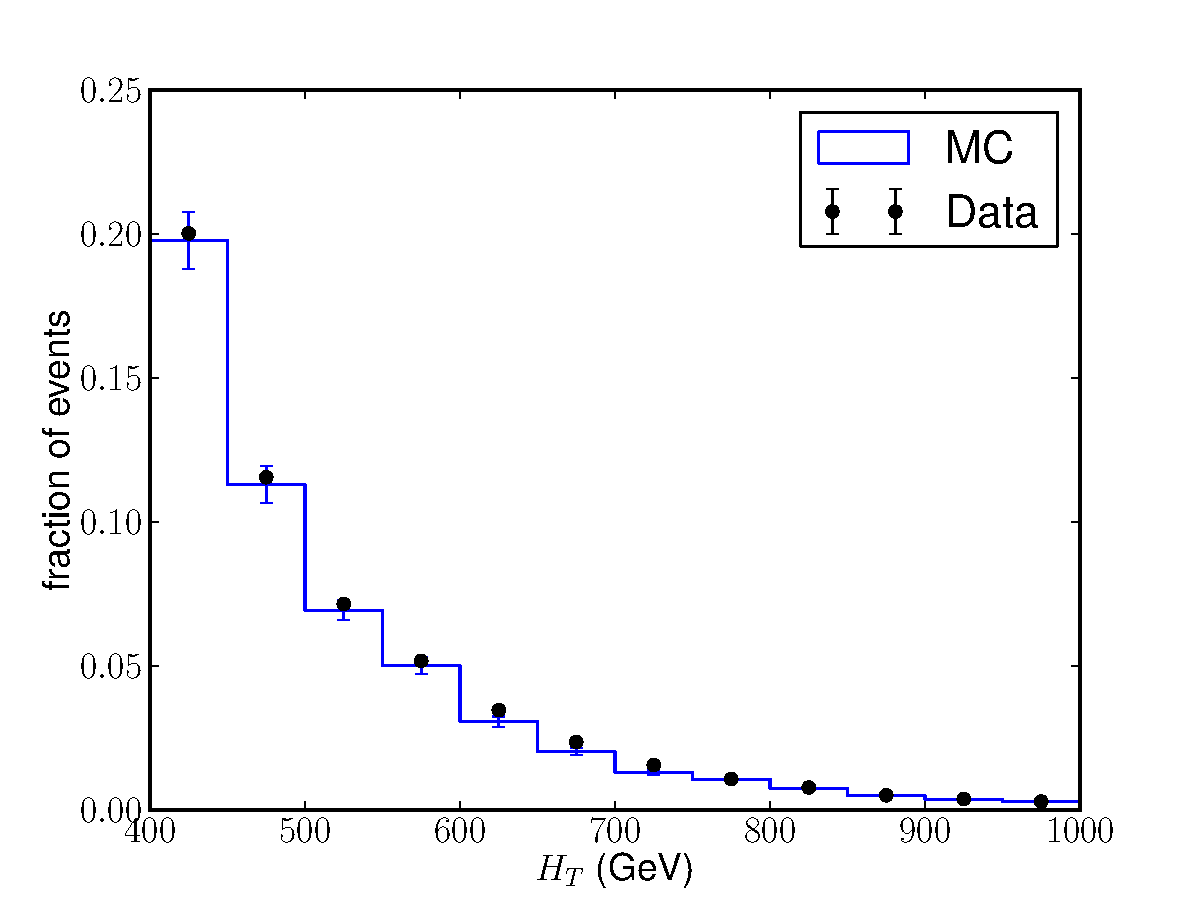
\includegraphics[width=0.5\textwidth]{Data_MC_HT.pdf}
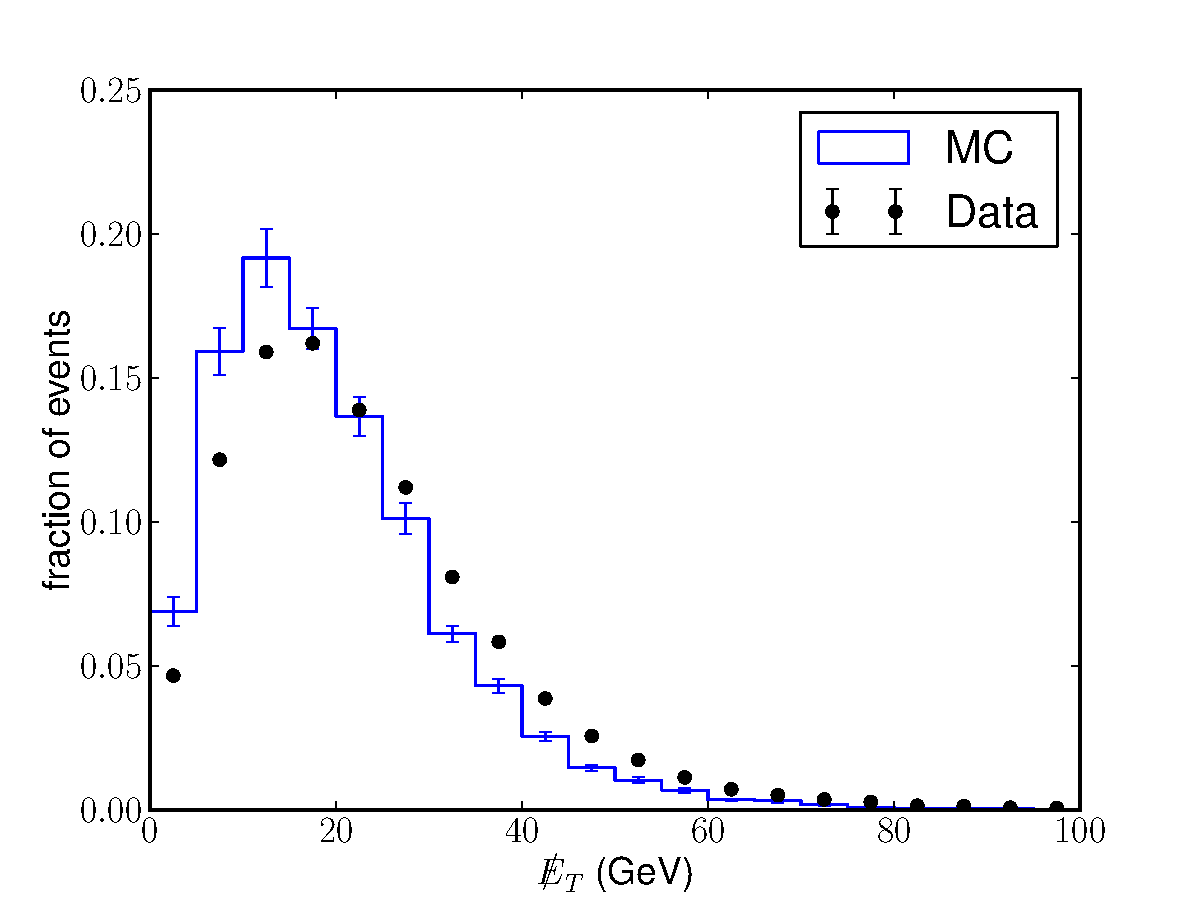
\includegraphics[width=0.5\textwidth]{Data_MC_MET.pdf}
\caption{Plots of $\HT$ and $\MET$ in data and Monte Carlo to show how accurately
the Monte Carlo models the data.}
\label{fig:Data_vs_MC}
\end{figure}

%Since the background estimation (see Section \ref{sec:QCD_Background}) is 
%largely data-driven the dependence of the result on Monte Carlo is limited.

\section{$\HT$ and Missing Transverse Energy ($\MET$)}

$\HT$ is the scalar sum of the $\pT$ of all jets with $\pT > 40\unit{GeV}$. The
$\HT$ gives a measure of the activity in the event.

\begin{equation}
\HT = \sum \pT^{jet}
\end{equation}

Particles such as neutrinos and the LSP in SUSY events are not detected by CMS.
Momentum conservation in the proton collision means that the undetected 
particles show up as an imbalance of reconstructed particles. $\MET$ is the
negative vector sum of the transverse momenta of all the reconstructed
particles. The transverse component is used because much of the longitudinal
momentum goes down the beampipe (i.e. outside the acceptance of the detector). 
For high energy photons and jets the most accurate measurement of the
momentum comes from the energy in the calorimeters. The transverse energy,
$\vec{E}_{T}$, of an energy deposit $E$ is calculated using Equation 
\ref{eq:et}. The missing transverse energy $\MET$ is given by Equation
\ref{eq:met}.

\begin{equation}
\vec{E}_{T} = E\sin{\theta}\cos{\phi}\vec{x} + E\sin{\theta}\sin{\phi}\vec{y}
\label{eq:et}
\end{equation}

\begin{equation}
\MET = \left| - \sum \vec{E}_{T} \right|
\label{eq:met}
\end{equation}

$\HT$ and $\MET$ are the two variables used to search for GMSB in the data.
Figures \ref{fig:susy_ht} and \ref{fig:susy_met} show the distribution of $\HT$ 
and $\MET$ in the signal events compared to the background from MC.

\begin{figure}
\begin{center}
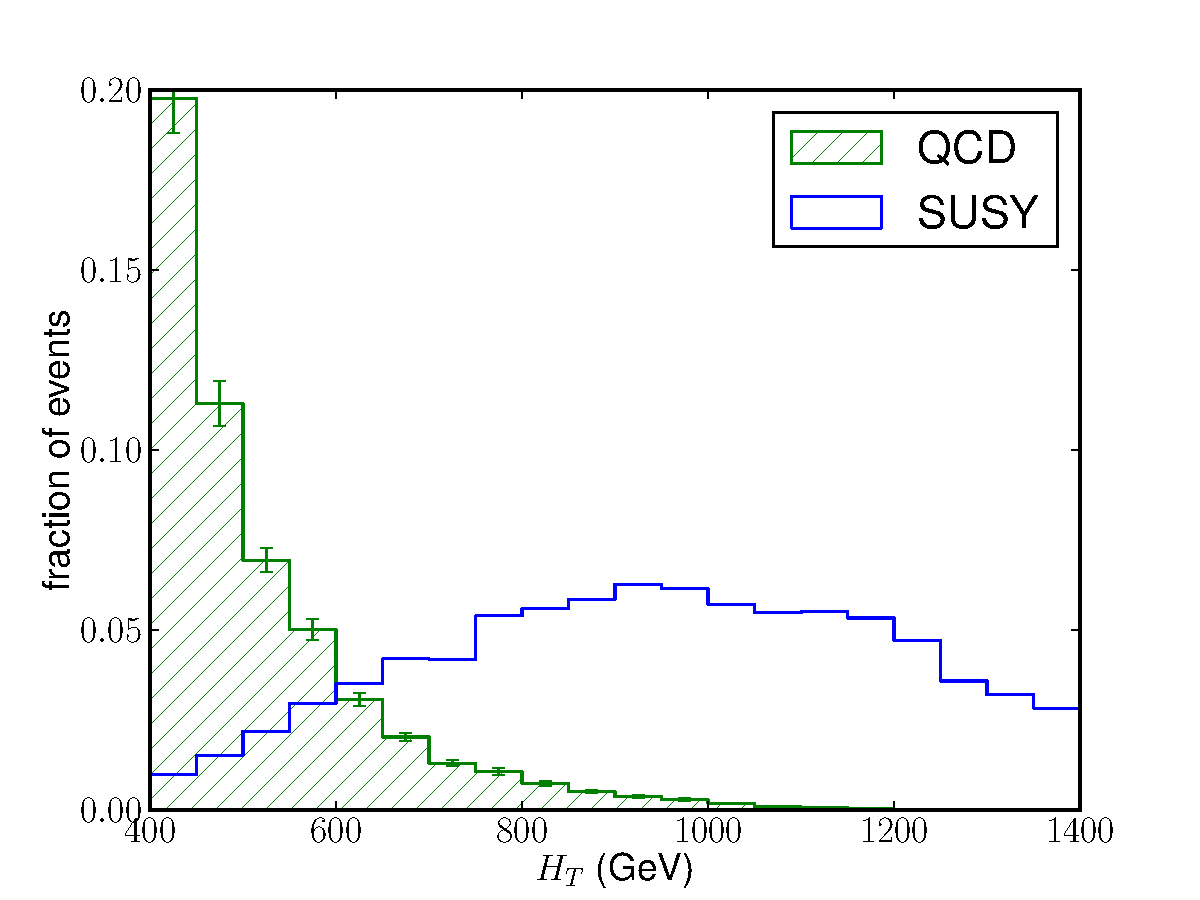
\includegraphics[width=0.8\textwidth]{SUSY_HT.pdf}
\end{center}
\caption{The $\HT$ distribution in SUSY events compared to the background from
MC samples.}
\end{figure} 

\begin{figure}
\begin{center}
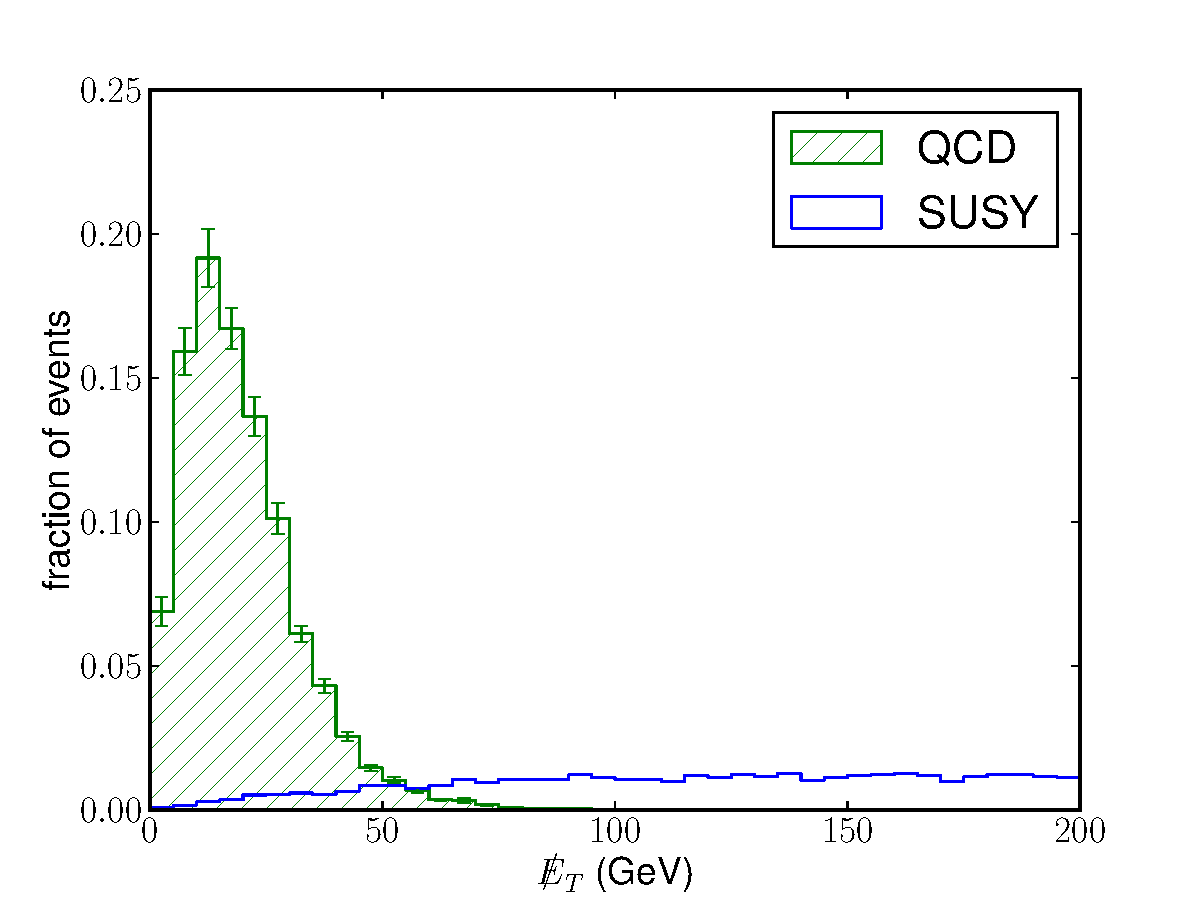
\includegraphics[width=0.8\textwidth]{SUSY_MET.pdf}
\end{center}
\caption{The $\MET$ distribution in SUSY events compared to the background from
MC samples.}
\end{figure} 

\section{Trigger}

Based on the properties of strong production GMSB, a photon + $\HT$ trigger 
is ideal for this search. Table \ref{tab:Triggers} shows a list of all the 
photon + $\HT$ triggers in the 2011 data with the corresponding L1 seed and the
rate at $10^{33}\unit{cm^{-2}s^{-1}}$. The 70\unit{GeV} photon + 350\unit{GeV}
$\HT$ trigger is used for this search. \\

\begin{table}
\begin{center}
\begin{tabular}{|l|c|c|}
\hline
 & L1 seed & Rate at $10^{33}\unit{cm^{-2}s^{-1}}$ \\
\hline
HLT\_Photon60\_CaloIdL\_HT200 & L1\_SingleEG20 & (pre-scaled) \\
HLT\_Photon70\_CaloIdL\_HT200 & L1\_SingleEG20 & (pre-scaled) \\
HLT\_Photon70\_CaloIdL\_HT300 & L1\_SingleEG20 & $4\unit{Hz}$ \\
HLT\_Photon70\_CaloIdL\_HT350 & L1\_SingleEG20 & $2.5\unit{Hz}$ \\
\hline
\end{tabular}
\end{center}
\caption{A table of the photon and $\HT$ triggers available in the 2011 data
along with the corresponding L1 seed and rate at $10^{33}\unit{cm^{-2}s^{-1}}$.}
\label{tab:Triggers}
\end{table}

As the luminosity has increased more stringent trigger requirements have been 
necessary to keep the data rate manageable. If the rate of a trigger becomes too
high, the trigger must be pre-scaled. This means that only every $n^{th}$ event 
which fires the trigger is read out where $n$ is the prescale factor. \\

An inefficiency of the trigger can come from a difference between the trigger 
and offline definitions of $\HT$ and photon $\pT$ caused by extra corrections
applied to the jets and the photons after the reconstruction. The offline cuts 
for $\HT$ and photon $\pT$ are chosen to avoid any inefficiency of the trigger 
due to the thresholds.

To evaluate the thresholds at which the trigger becomes efficient, the
efficiency of the trigger is evaluated with respect to a lower threshold 
trigger. Data ranges are selected such that the two triggers are both in the
menu and the higher threshold trigger is unprescaled. To evaluate the trigger
efficiency as a function of $\HT$ the $\HT$ distribution of events passing both
triggers is divided by the $\HT$ distribution of events passing the lower
threshold trigger. The efficiency curve tells us where to put the off-line cut 
in $\HT$ such that the trigger is fully efficient. Figure 
\ref{fig:Trigger_Efficiency} shows the trigger efficiency against $\HT$ and 
photon $\pT$.

\begin{figure}
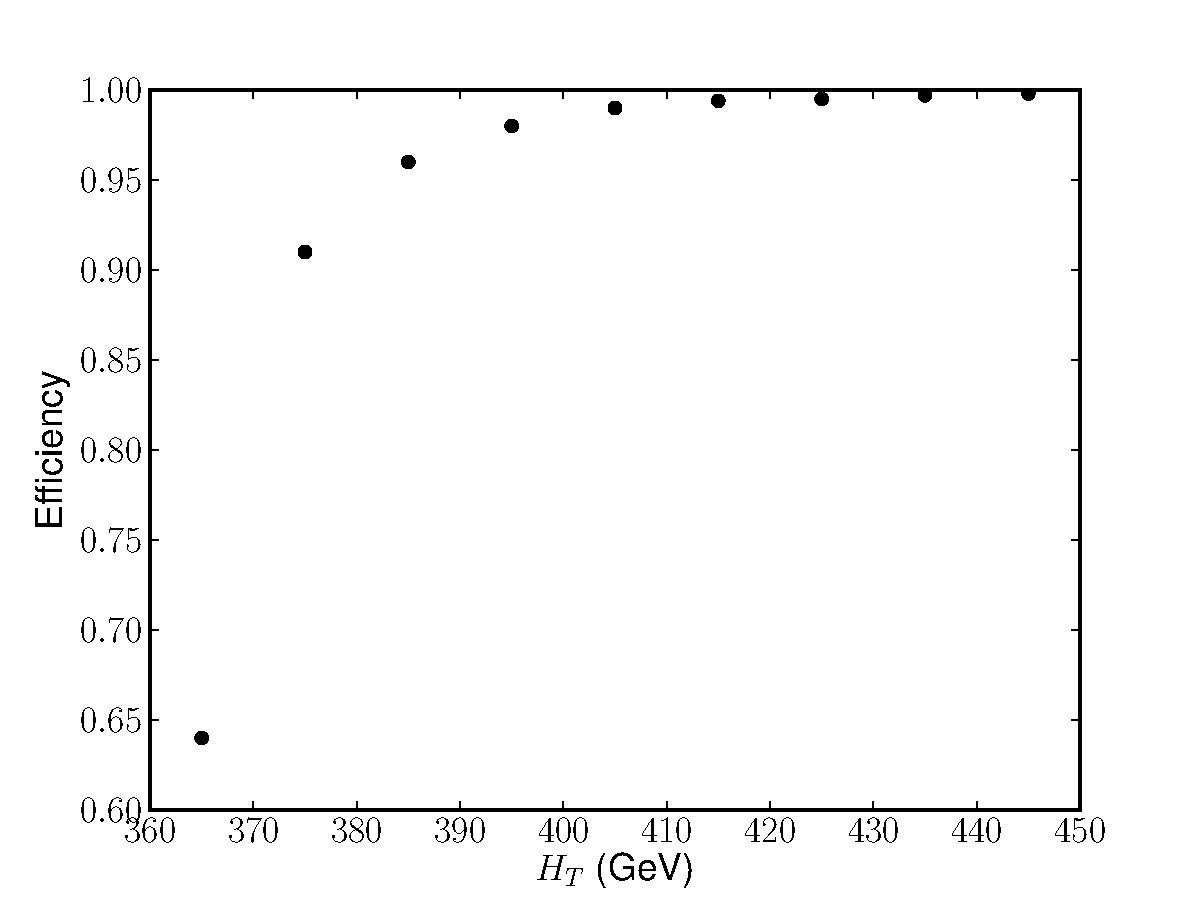
\includegraphics[width=0.5\textwidth]{Trigger_Efficiency_HT.pdf}
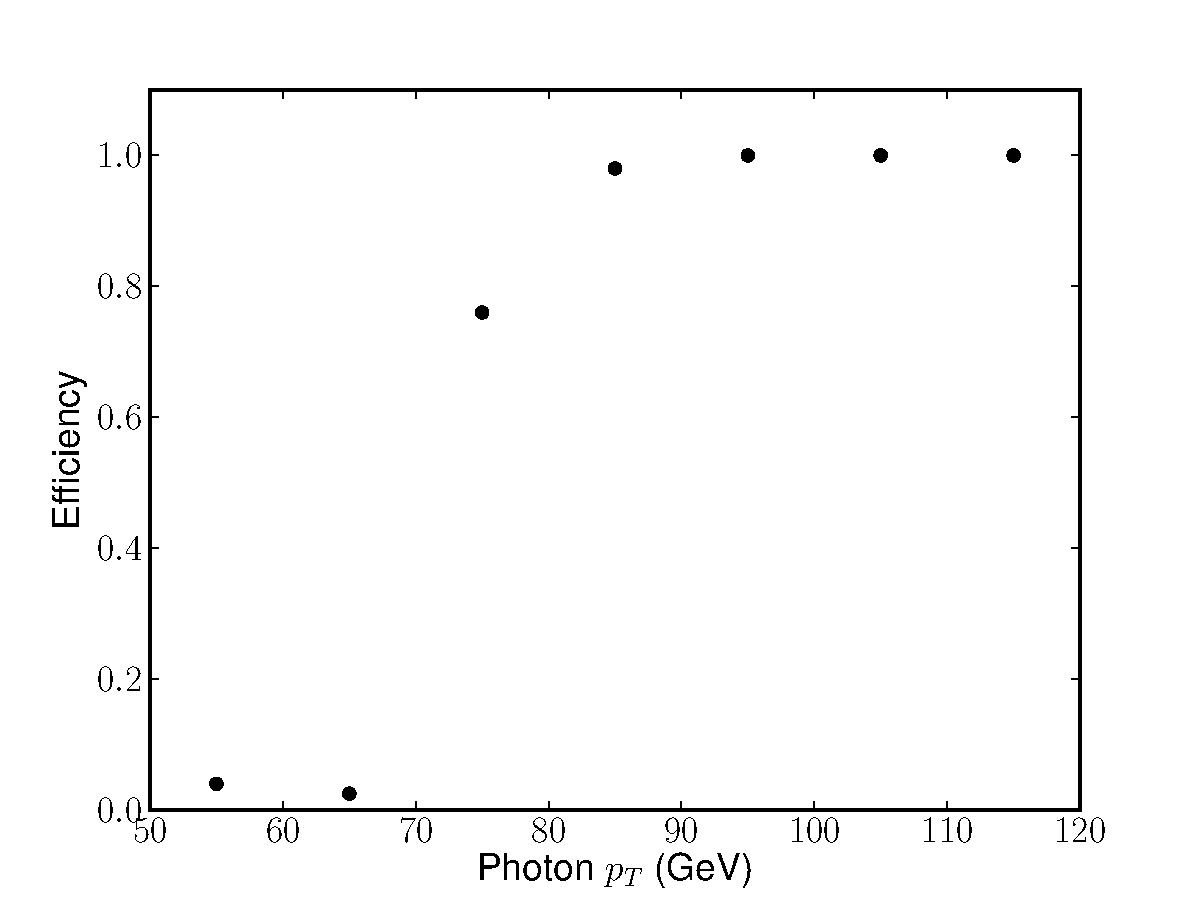
\includegraphics[width=0.5\textwidth]{Trigger_Efficiency_PhotonPt.pdf}
\caption{The trigger efficiency vs $\HT$ (left) and vs photon $\pT$ (right)
relative to a lower threshold trigger.}
\label{fig:Trigger_Efficiency}
\end{figure}

\section{Photon Selection}

Photons are selected based on variables such as isolation and shower shape which
are designed to select prompt photons over fakes from jets. The photon 
reconstruction is described in detail in Section \ref{sec:photon_recontruction}. 
The cut values on each of the photon selection varaibles are listed in Table 
\ref{tab:photoncuts}. These cut values were chosen to have 90\unit{\%} efficiency
for prompt photons according to MC \cite{photon_cuts}.

\begin{table}
\begin{center}
\begin{tabular}{|c|c|}
\hline
Variable & Cut value \\
\hline
ECAL isolation & $4.2 + 0.006\pT$ \\
HCAL isolation & $2.2 + 0.0025\pT$ \\
Track isolation & $2.0 + 0.001\pT$ \\
H/E & 0.05 \\
Shower Shape & 0.012 (EB), 0.030 (EE) \\
No Pixel Seed & True \\
\hline
\end{tabular}
\end{center}
\caption{The photon selection cuts.}
\label{tab:photoncuts}
\end{table}

\section{Jet Selection}

Two jets with $\pT > 80 \unit{GeV}$ and $|\eta| < 2.5$ are required. The $\eta$
threshold corresponds to the tracker boundary. The $\pT$ threshold should be
chosen as high as possible to reject background, but with the signal efficiency
close to 100\%. Figure \ref{fig:Jet_Threshold} shows the signal efficiency and 
the background rejection as a function of the jet $\pT$ threshold. 

\begin{figure}
\begin{center}
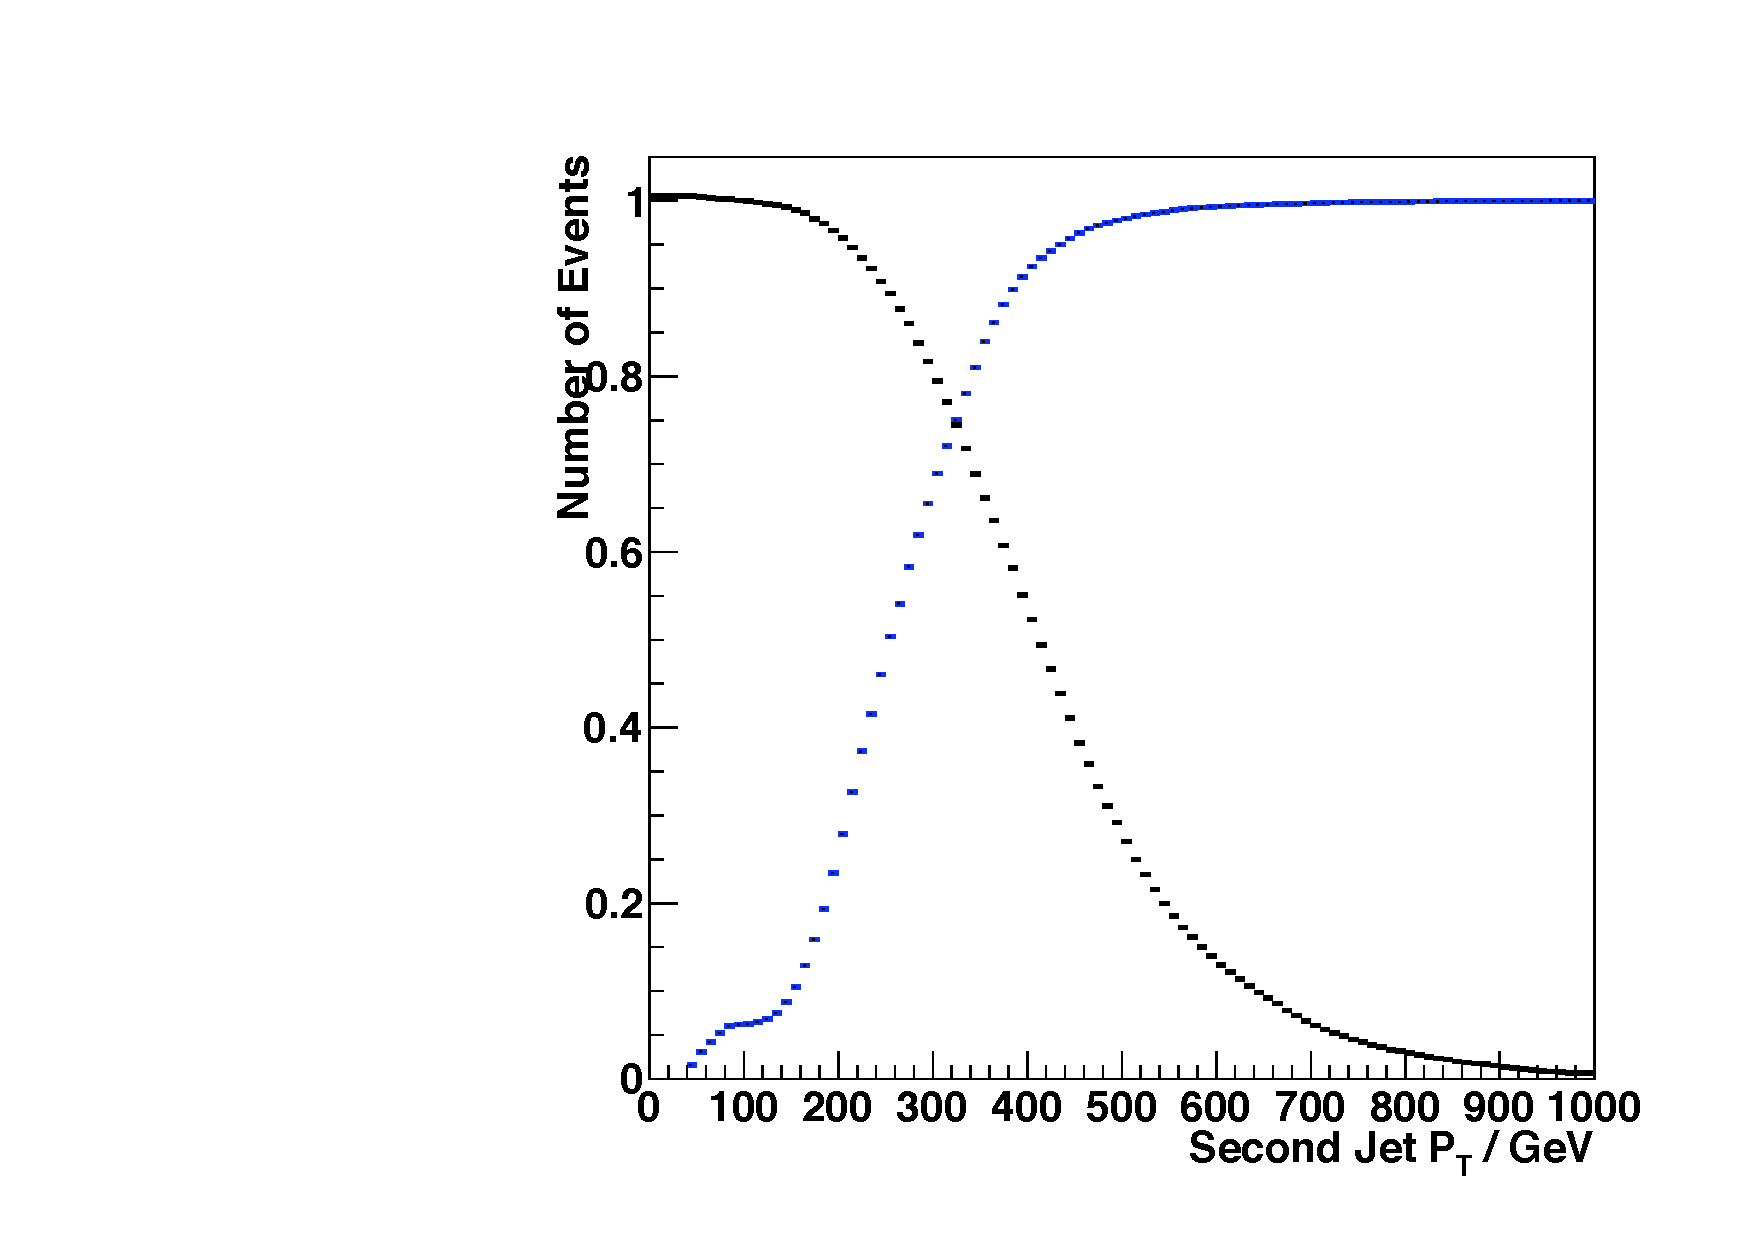
\includegraphics[width=0.7\textwidth]{Jet_Threshold.pdf}
\end{center}
\caption{A plot of the efficiency of the signal (black) and the background
rejection (blue) as a function of the jet $\pT$ threshold.}
\label{fig:Jet_Threshold}
\end{figure}

\section{Event Selection}
\label{sec:Event_Selection}

The event selection criteria are listed below. 

\begin{itemize}
\item $\HT > 400 \unit{GeV}$
\item $\geq 2$ jets
\item $\geq 1$ photon
\item $\MET > 50 \unit{GeV}$
\end{itemize}

A $\HT$ cut is applied because strongly production SUSY events have high $\HT$
since high mass particles (squarks and gluinos) are produced. The value of this 
cut is motivated by the desire for the trigger to be fully efficiency for the 
event selection. Figure \ref{fig:Trigger_Efficiency} shows that the trigger 
becomes fully efficient in $\HT$ at around $400\unit{GeV}$. \\

The $\geq 2$ jets cut is well motivated from the SUSY perspective: strong
production SUSY events start with two squarks/gluinos each of which decay to a 
quark/gluon (which forms a jet in the detector) and the next SUSY particle in 
the mass hierarchy. \\

In strong production GMSB the Next-to-Lightest SUSY Particle (NLSP) is the 
neutralino ($\tilde{\chi}^{0}$) which decays to a photon and a gravitino. At 
least two photons are expected in each event. However, due to the high activity 
in these events, photons often fall inside the cone of a jet and so only one 
photon is reconstructed. Hence the $\geq 1$ photon cut. \\

The background estimation is done in bins of $\MET$ and $\HT$, but an initial 
$\MET$ cut is made to avoid the low $\MET$ bins where there is no sensitivity 
due to the huge amount of background. Figure \ref{fig:met_threshold} shows the 
signal efficiency and the background rejection as a function of $\MET$ cut.

\begin{figure}
\begin{center}
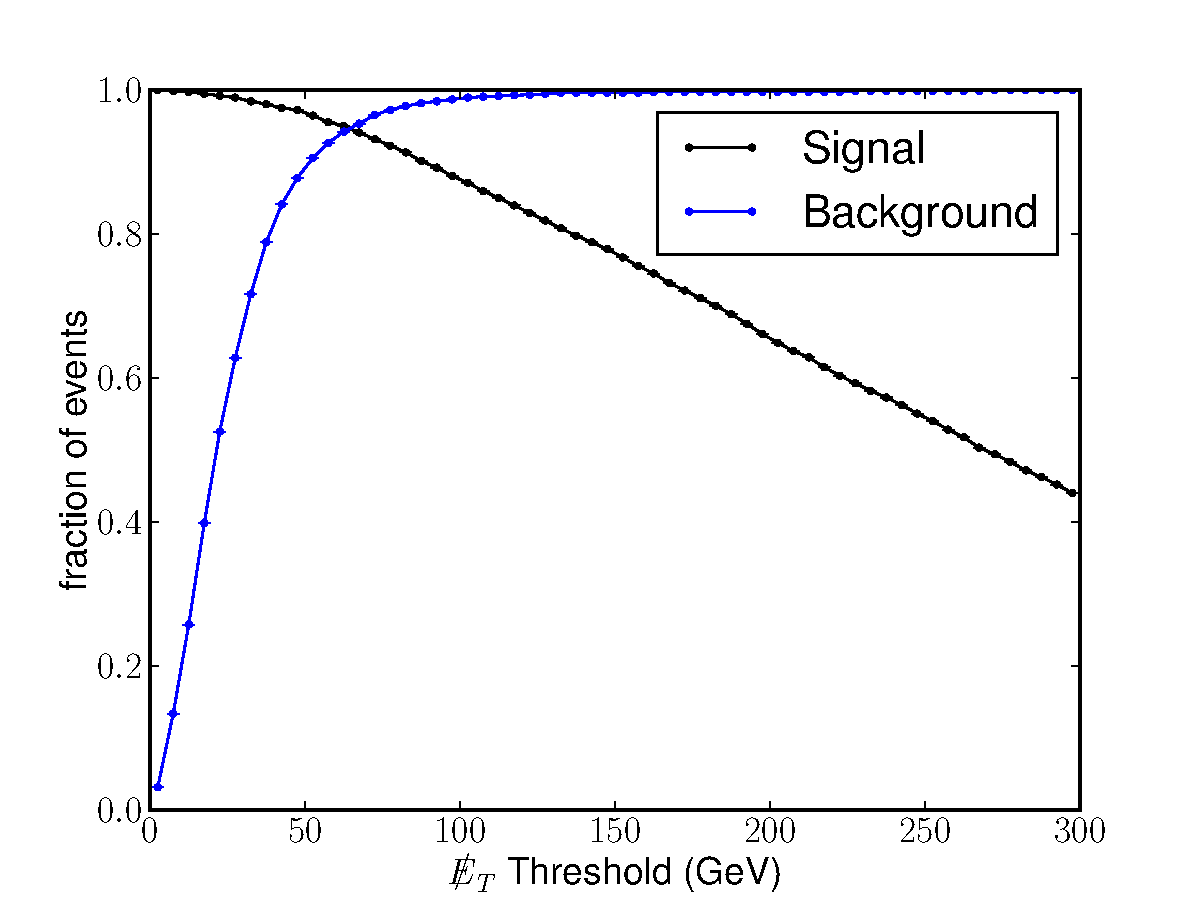
\includegraphics[width=0.7\textwidth]{MET_Threshold.pdf}
\end{center}
\caption{The signal efficiency (black) and background rejection (blue) as a
function of $\MET$ cut.}
\label{fig:met_threshold}
\end{figure}

The total number of events passing the selection in bins of $\HT$ and $\MET$ is
given in Table \ref{tab:events}.

\begin{table}
\begin{center}
\begin{tabular}{|c|c|c|c|c|}
\hline
$\MET\downarrow | \HT\rightarrow$ & $400-500\unit{GeV}$ & $500-600\unit{GeV}$ 
& $600-700\unit{GeV}$ & $700\unit{GeV}+$ \\ 
\hline
$50-100\unit{GeV}$ & 835 & 591 & 398 & 609 \\
\hline
$100-150\unit{GeV}$ & 35 & 30 & 26 & 44 \\
\hline
$150-200\unit{GeV}$ & 5 & 5 & 2 & 7 \\
\hline
$200\unit{GeV}+$ & 9 & 4 & 4 & 7 \\
\hline
\end{tabular}
\end{center}
\caption{The number of events passing the selection in bins of $\HT$ and $\MET$.}
\label{tab:events}
\end{table}

\section{Outline of the Search}

The event selection is applied to the data and the number of events passing the
selection is recorded in bins of ($\HT$, $\MET$). \\

An estimate is made for the expected number of background events in each ($\HT$,
$\MET$) bin. The background estimation is done using a sample from data and
checked using the MC. \\

A prediction for the number of signal events in the only significant bin 
($\HT>700\unit{GeV}$, $\MET>200\unit{GeV}$) is made by applying the event
selection to the signal MC. The prediction is made for a variety of signal 
models with different squark mass and gluino mass. Systematic uncertainties are 
estimated by varying within their uncertainties the variables that could affect 
the signal prediction. \\

The CLs method is used to exclude the signal at 95\unit{\%} CL in the squark
mass vs gluino mass parameter space.
